\subsection{The Halved Model}
\label{sec:add.add.halved}

The idea behind the halved model is that the model we have can be looked at differently than it was introduced in.
We know the model $m$ maps an input $x$ to $f(x) \mod 1$, meaning that if the output $f(x)$ is greater or equal to 1, we subtract 1 from it until it is in the range $[0, 1)$.
Similarly, we add 1 to it if it is smaller than 0 until it is in the desired range.
Now instead of confining the model to the domain of $[0, 1)$, we think of it repeating infinitely in both directions.
This process is called lifting of circle maps and is described by \Citeauthor{devaney2021introduction} in his book~\cite{devaney2021introduction}.
We can achieve this by mapping $T^m: x \mapsto f(x - \lfloor x \rfloor)$.
This trick maps the input $x$ into the domain, on which our model function produces sensible results and causes it to repeat infinitely.
$T^m$ is now a lift of the model $m$ in the domain of all real numbers $\mathbb{R}$.
\Cref{fig:minrep.infinite.model.concept} illustrates this concept for the cycle $P_7^3$.
The blue square is the full model.
One can see, that the branch $f_\D$ is outside the blue square at its right edge.
This is because it was cut off and continued at the bottom of the square before, due to the $\mod 1$ operation.

\todo{This makes sense in the original problem domain}

In this model, there are no cycles that have multiple rotations.
Instead, the cycles that had multiple rotations in the full model, manifest as a sequence of different blocks of the full model.
Meaning for the example $P_7^3$, the same blocks of $\A^4\B^3\C^4\D^3$ are repeating infinitely.
But for an example with multiple rotations, such as $\A\B\C\D\A^2\B^2\C^2\D^2$, the blocks will not all be the same.
Instead, the blocks $\A\B\C\D$ and $\A^2\B^2\C^2\D^2$ will be alternating.

Now the symmetry of our function $f$ comes into play.
Since $f(x + 0.5) = f(x) + 0.5$ for $x \in [0, 0.5)$, we can split the infinite model into smaller blocks than the blue block of the full model.
The function of the infinite model repeats in blocks of size 0.5, these blocks are marked red in \Cref{fig:minrep.infinite.model.concept}.
These red blocks represent the halved model, it is the smallest repeating part of the infinite model $T^m$.
Basically we choose the smallest model, of which $T^m$ is a lift.
This happens to be exactly our model $m$ folded in half.
Se the halved model $h$ is defined on the interval $[0, \frac{1}{2})$ and maps $x \mapsto g(x) \mod \frac{1}{2}$, where $g(x)$ is the same as in our model $m$, defined in \Cref{sec:minrep.definition}.

To get the symbolic sequence of a cycle in the halved model, we look at the pattern in which different red blocks repeat along the infinite model.
For our example in the picture, there is only one red block that repeats infinitely, $\L^4\R^3$.
The next section will explain, how to translate cycles between the halved and full model.

\begin{figure}
	\centering
	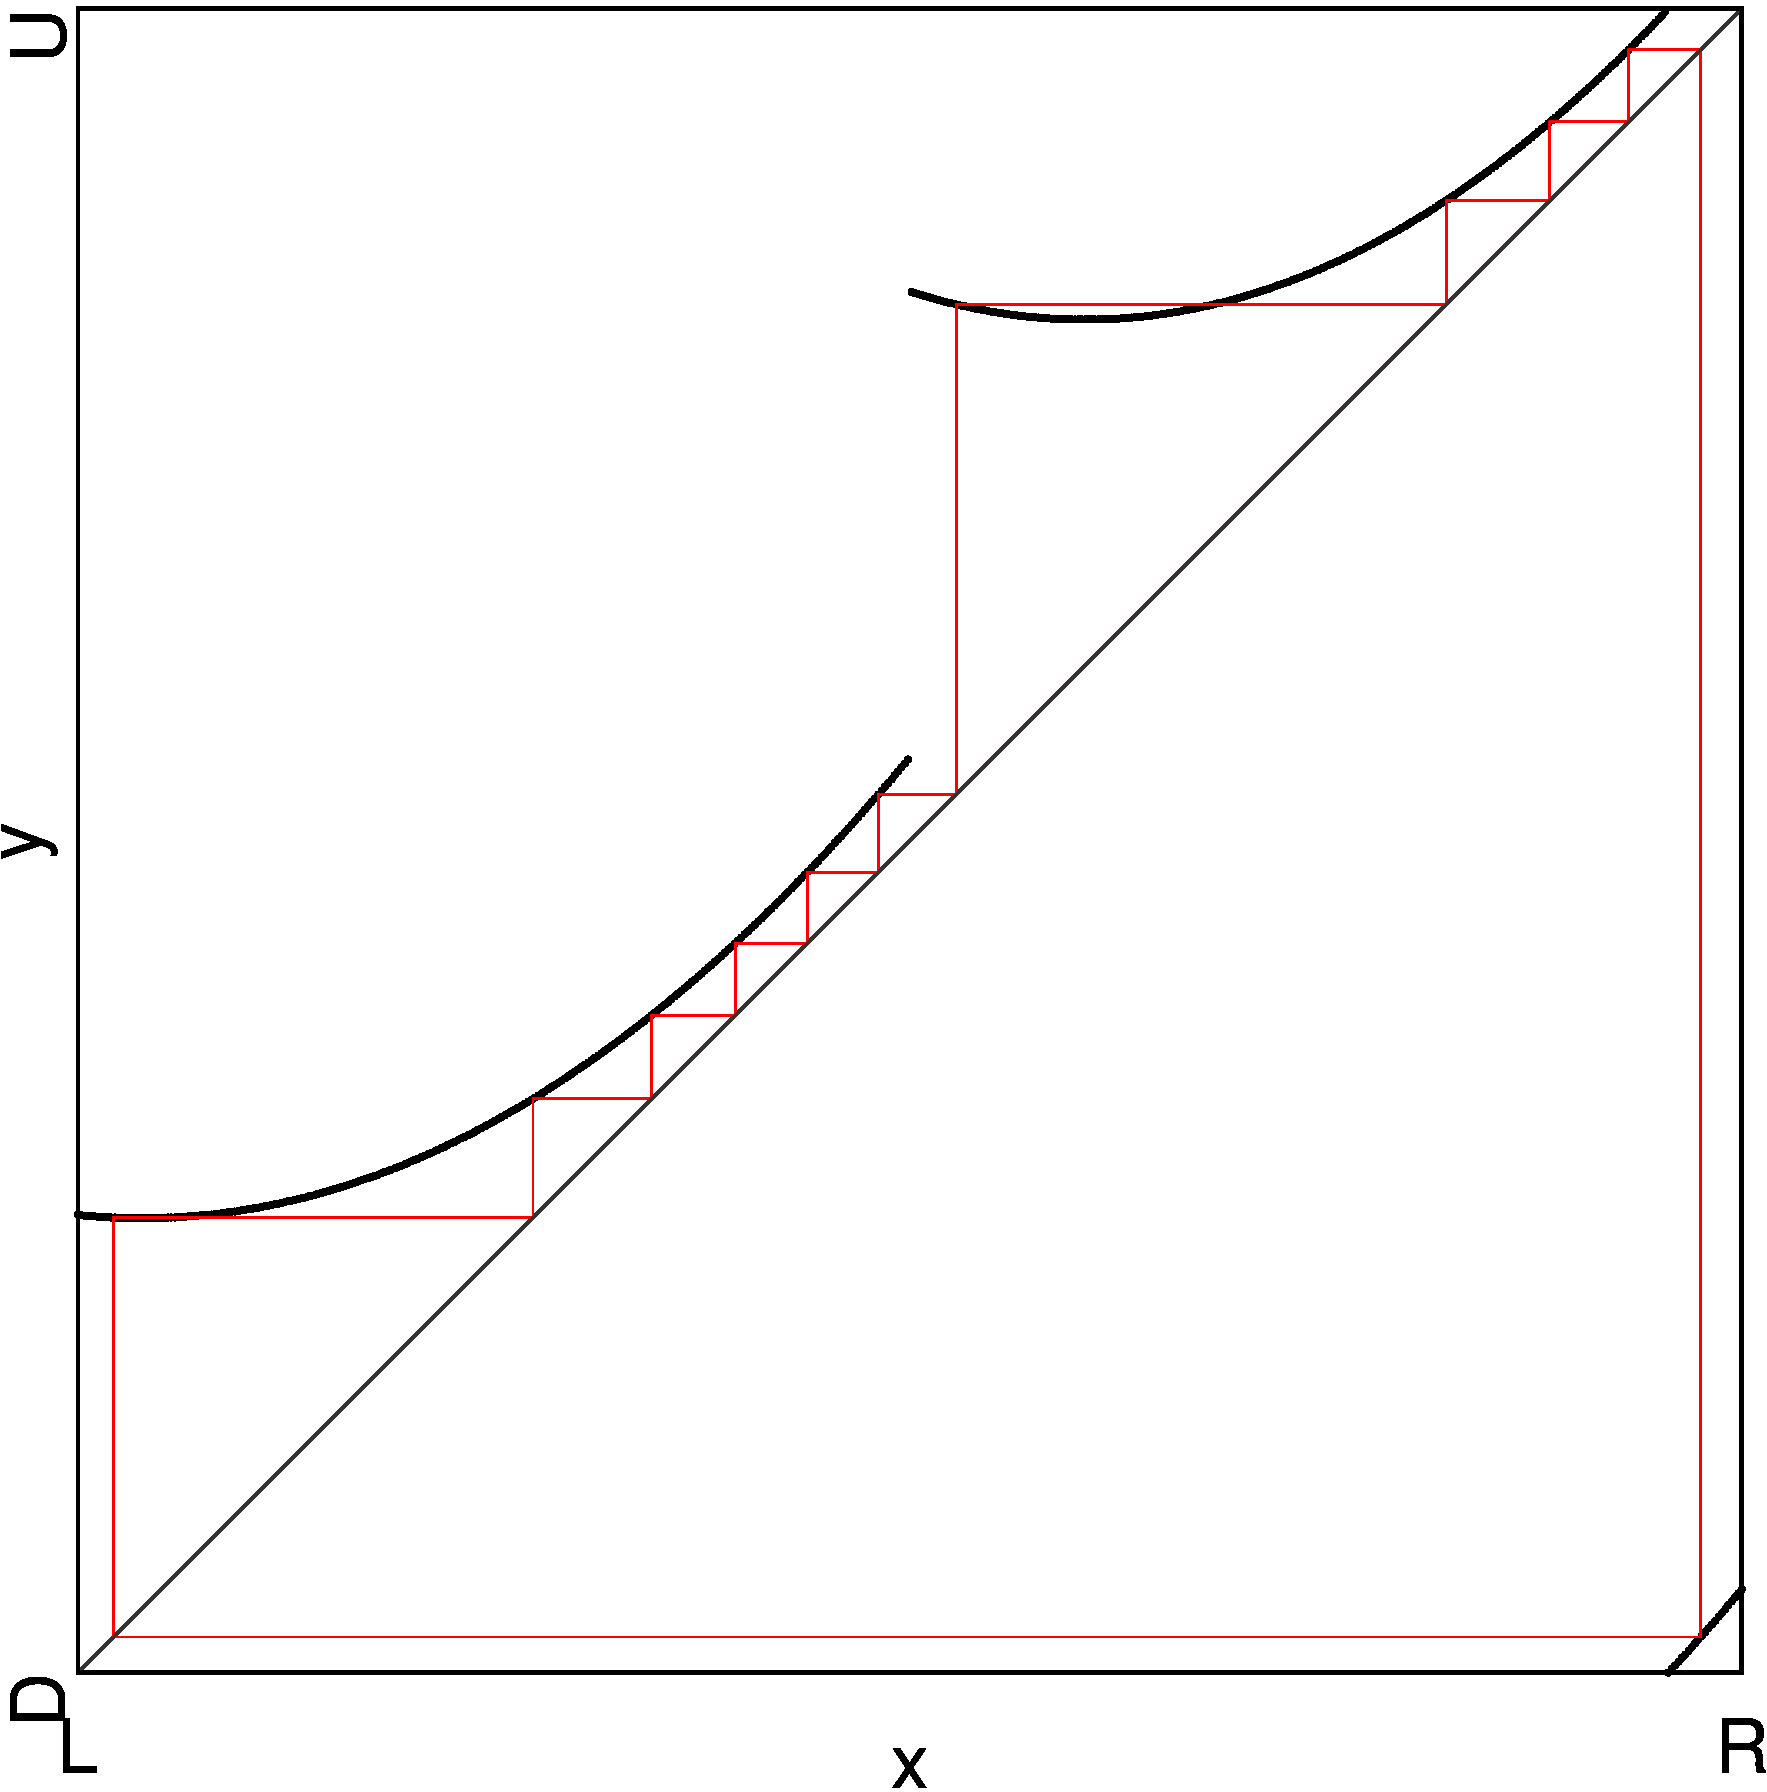
\includegraphics[width=.7 \textwidth]{63_MinimalRepr_Adding_Halved/Cob_Vis_s/Manual/result.png}
	\caption{Illustration of the infinite model concept.}
	\label{fig:minrep.infinite.model.concept}
\end{figure}

\begin{figure}
	\centering
	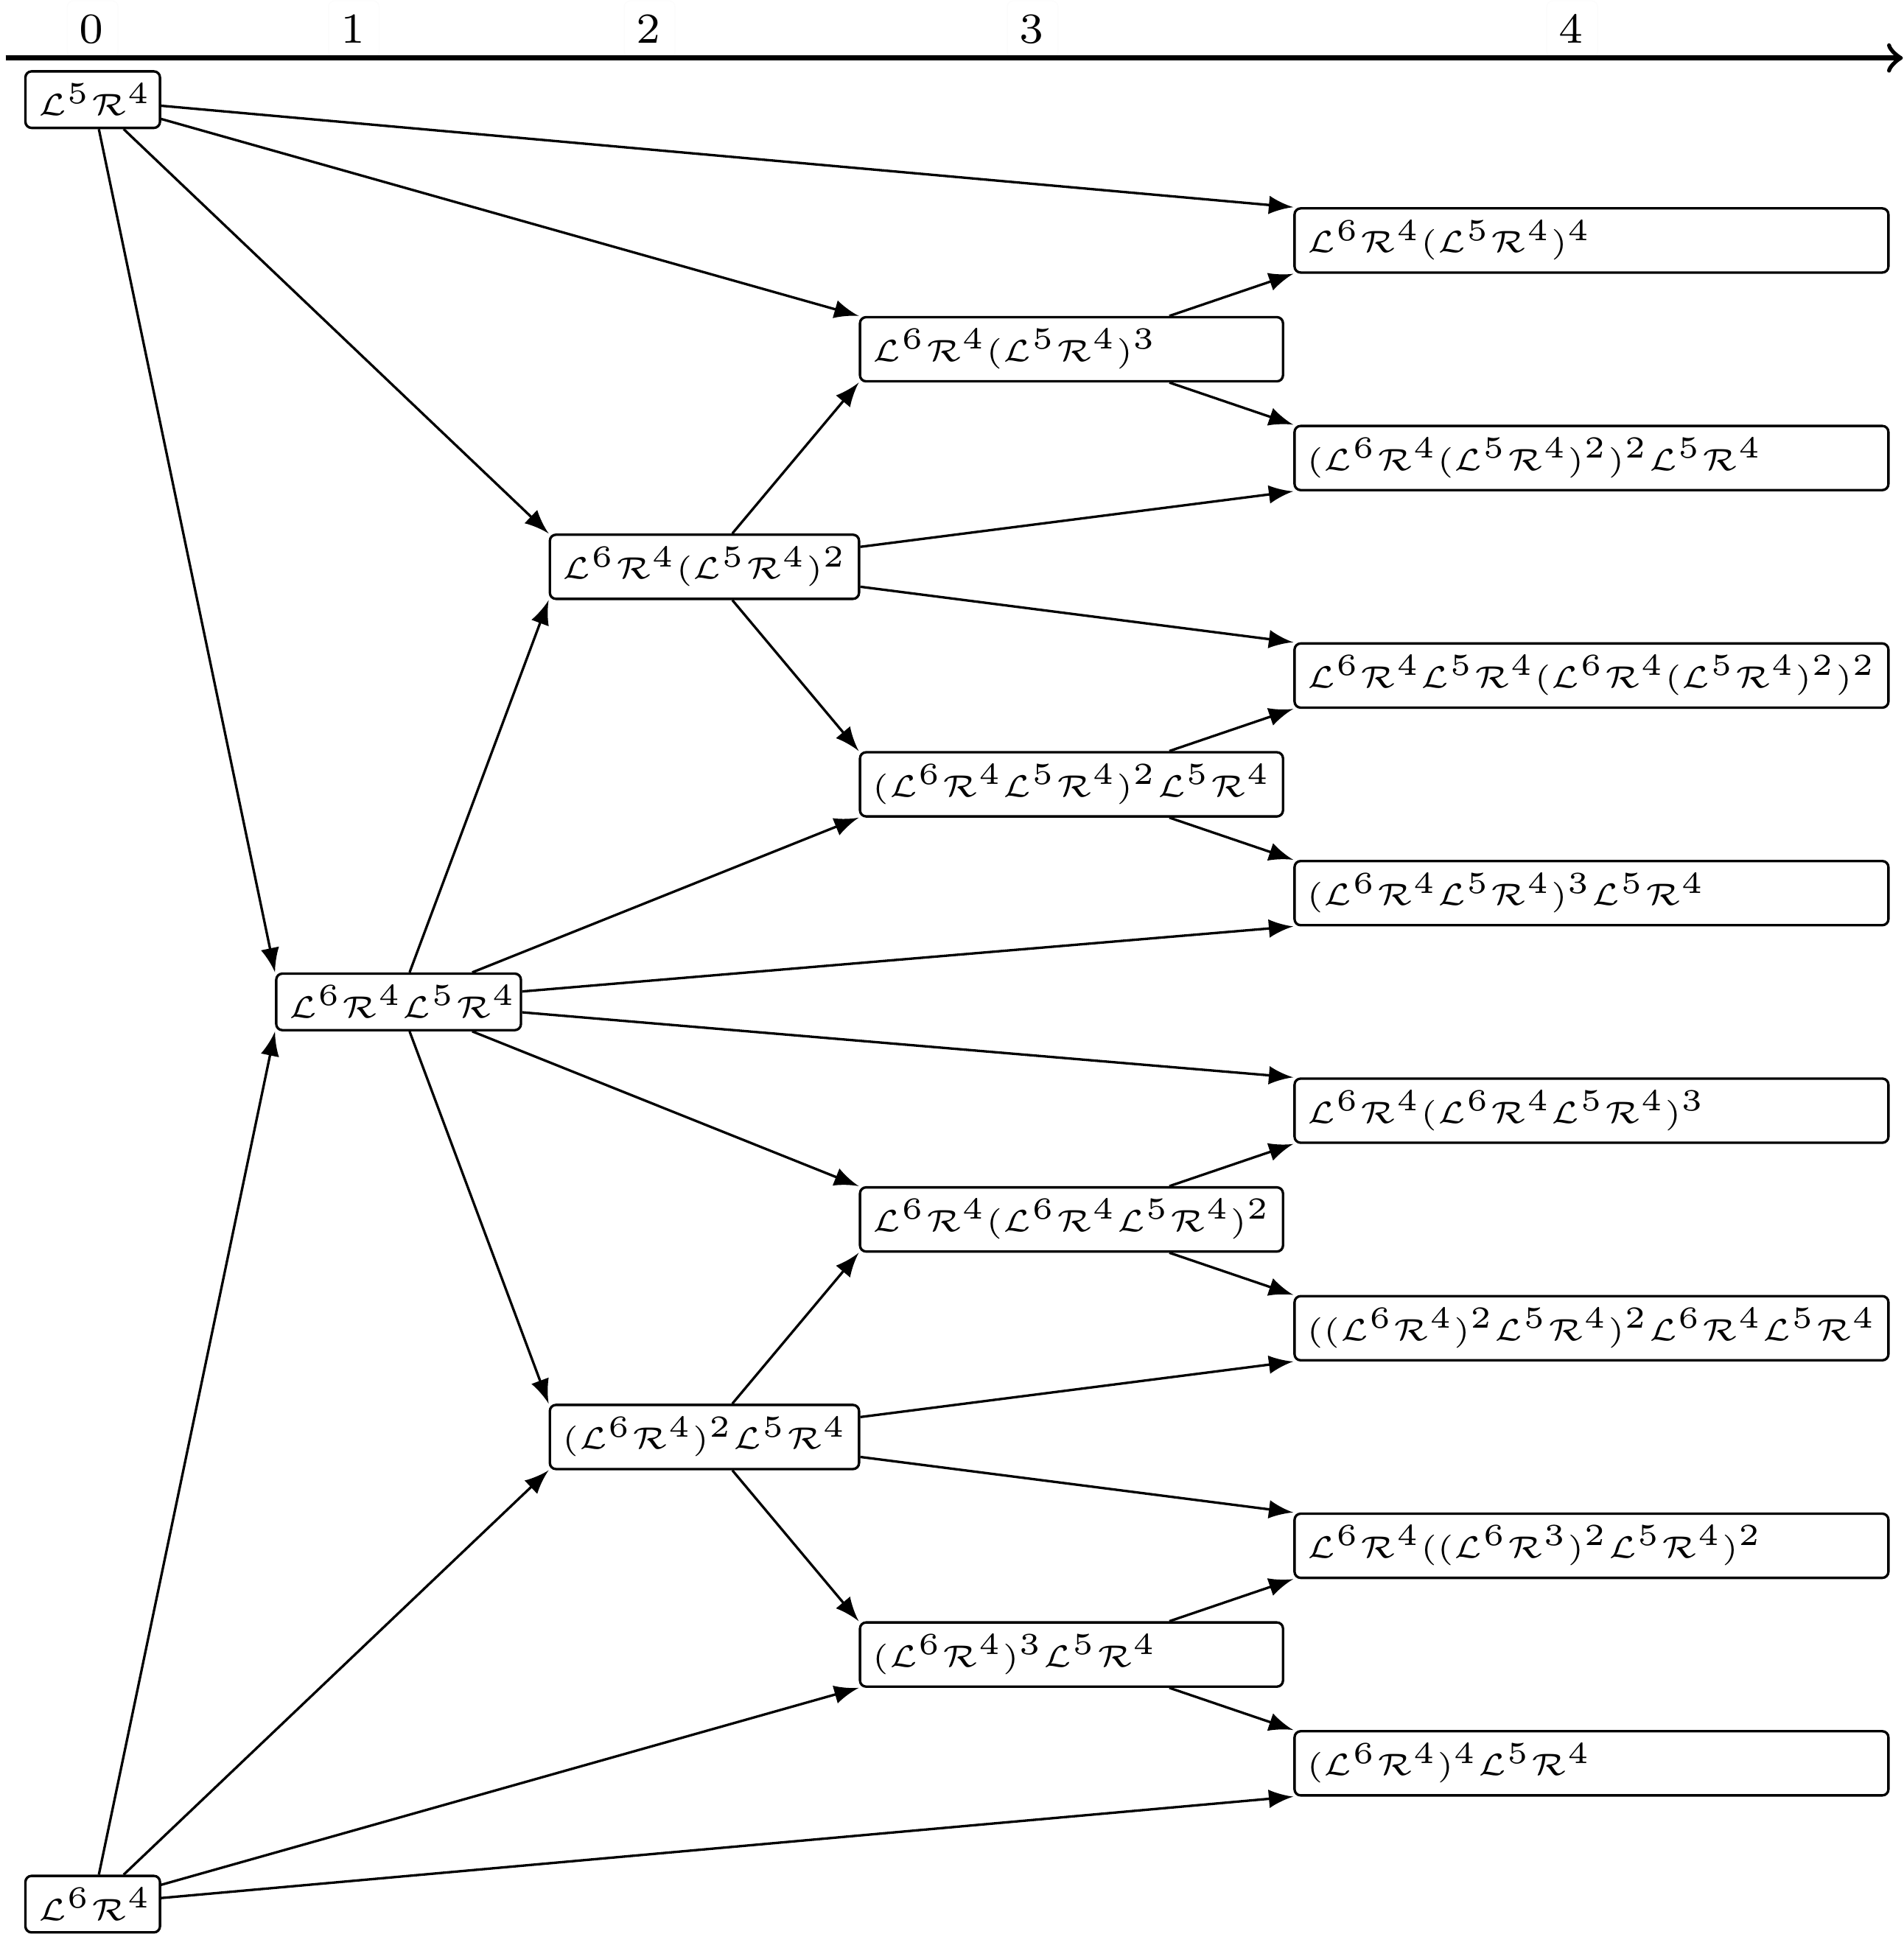
\includegraphics[width=\textwidth]{FareyTrees/Minrep_Adding1_Halved/adding.png}
	\caption{t}
	\label{fig:tree.adding1.hor.halved}
\end{figure}
